\documentclass[14pt,a4paper]{scrartcl}
\usepackage{cmap}
\usepackage[utf8]{inputenc}
\usepackage[T1,T2A]{fontenc}
\usepackage[english,russian]{babel}
\usepackage{relsize}
\usepackage{graphicx}
\usepackage{subfigure}
\usepackage{mathtools}
\usepackage{amssymb}
\usepackage{float}
\usepackage{sidecap}
\usepackage{wrapfig}
\usepackage{caption}
\usepackage[table,xcdraw]{xcolor}
\usepackage{listings}
\usepackage{amsmath,cryptocode}
\usepackage{listings}
\usepackage{booktabs}
\usepackage{multirow}  
\usepackage{multicol}
\usepackage{bigstrut}
\usepackage{lscape}
\usepackage{rotating}
\usepackage{adjustbox}
\usepackage{minted}
\usepackage{breqn}
\usepackage{physics}


\newcommand\scalemath[2]{\scalebox{#1}{\mbox{\ensuremath{\displaystyle #2}}}}


\begin{document}
	\begin{titlepage}
	\begin{center}
		\large
		МИНИСТЕРСТВО ОБРАЗОВАНИЯ И НАУКИ\\ РОССИЙСКОЙ ФЕДЕРАЦИИ
		
		\vspace{0.5cm}
		
		МГТУ им Н.Э.Баумана
		\vspace{0.25cm}
		
		Факультет ФН
		
		Кафедра вычислительной математики и математической физики
		\vfill
		
		
		Соколов Арсений Андреевич\\
		\vfill
		
		
		{\LARGE Домашнее задание №3 по основам сеточных методов \\[2mm]
		}
		\bigskip
		
		3 курс, группа ФН11-63Б\\
		Вариант 3
	\end{center}
	\vfill
	
	\newlength{\ML}
	\settowidth{\ML}{«\underline{\hspace{0.7cm}}» \underline{\hspace{2cm}}}
	\hfill\begin{minipage}{0.4\textwidth}
		Преподаватель\\
		\underline{\hspace{3cm}} В.\,А.~Кутыркин\\
		«\underline{\hspace{0.7cm}}» \underline{\hspace{1.71cm}} 2020 г.
	\end{minipage}%
	\bigskip
	
	
	\vfill
	
	\begin{center}
		Москва, 2020 г.
	\end{center}
\end{titlepage}

\section*{Задание 1}
\textbf{Задание.}\\

Используя метод Рунге-Кутты порядка $m = 4$, четырёхшаговый метод Адамса-Башфорта и метод прогноза-коррекции (с четвёртым порядком точности) найти численные решения задачи Коши (шаг сетки $h = 0.05$):

\begin{equation*}
	\left\{\begin{array}{l}
	\frac{d x}{d t}=\frac{2 N+3}{N+(n-60)+1} \sin \left(\frac{2 N+3}{(N+n-60) \cdot t} x\right), \quad t \in[0.5 ; 2.5] \\
	x(0.5)=\frac{N}{4}
	\end{array}\right.
\end{equation*}

Графически проиллюстрировать сравнение приближённых решений. Используя практическое правило Рунге, оценить погрешность приближённого решения по методу Рунге-Кутты порядка $m=4$.

\textbf{Решение.}\\

Подставим значения $n = 63, N = 3$ в систему:

\begin{align*}
	&\dv{t}x(t) = {\frac {\rm d}{{\rm d}t}}x \left( t \right) ={\frac {9}{7}\sin \left( 
		3/2\,{\frac {x \left( t \right) }{t}} \right) }	\\
	&x(0.5) = \frac{3}{4}
\end{align*}


\section{Метод Рунге-Кутты порядка $m=4$}

Равномерную сетку задаём $\frac{b-a}{h}+1 = \frac{2.5-0.5}{0.05} + 1 = 41$ узлами. При $m = 4$ используется рабочая формула вида:

\begin{equation*}
	\left\{\begin{array}{l}
	x_{0}(t+h)=x_{0}(t)+\frac{h}{6}\left(\omega_{1}+2 \omega_{2}+2 \omega_{3}+\omega_{4}\right)+O\left(h^{5}\right) \\
	\omega_{1}=\omega_{1}\left(t, x_{0}(t), h\right)=f\left(t, x_{0}(t)\right) \\
	\omega_{2}=\omega_{2}\left(t, x_{0}(t), h\right)=f\left(t+\frac{1}{2} h, x_{0}(t)+\frac{1}{2} h \omega_{1}\right) \\
	\omega_{3}=\omega_{3}\left(t, x_{0}(t), h\right)=f\left(t+\frac{1}{2} h, x_{0}(t)+\frac{1}{2} h \omega_{2}\right) \\
	\omega_{3}=\omega_{3}\left(t, x_{0}(t), h\right)=f\left(t+h, x_{0}(t)+h \omega_{3}\right)
	\end{array}\right.
\end{equation*}

Тогда

\begin{align*}
	^>x^0 &= [3/4, 0.8075773070, 0.8658126486, 0.9245493314, 0.9836782141,
	1.043120710, \\& 1.102818639, 1.162727898, 1.222814372, 1.283051205,
	1.343416927, \\& 1.403894142, 1.464468582, 1.525128421, 1.585863759,
	1.646666238, \\& 1.707528745, 1.768445184, 1.829410293, 1.890419506,
	1.951468836, \\& 2.012554786, 2.073674272, 2.134824563, 2.196003230,
	2.257208106, \\& 2.318437249, 2.379688912, 2.440961521, 2.502253652,
	2.563564014, \\& 2.624891431, 2.686234831, 2.747593236, 2.808965748,
	2.870351544, \\& 2.931749865, 2.993160014, 3.054581345, 3.116013262,
	3.177455211]
\end{align*}





\section*{Четырёхшаговый метод Адамса-Башфорта}
Первые четыре значения $^>x^1$ найдены методом Рунге-Кутты порядка $m=4$

\begin{equation*}
	x_{n+1}=x_{n}+\frac{h}{24}\left(55 f_{n}-59 f_{n-1}+37 f_{n-2}-9 f_{n-3}\right),
\end{equation*}

где $f_i = f(t_i,x_i)$


Тогда


\begin{align*}
	^>x^1 &= [3/4, 0.8075773070, 0.8658126486, 0.9245493314, 0.9836861018,
	1.043132300, \\& 1.102832799, 1.162743180, 1.222830266, 1.283067324,
	1.343433075, \\& 1.403910189, 1.464484454, 1.525144073, 1.585879167,
	1.646681390, \\& 1.707543637, 1.768459816, 1.829424670, 1.890433634,
	1.951482723, \\& 2.012568439, 2.073687700, 2.134837774, 2.196016232,
	2.257220907, \\& 2.318449856, 2.379701333, 2.440973764, 2.502265723,
	2.563575919, \\& 2.624903176, 2.686246422, 2.747604678, 2.808977047,
	2.870362704, \\& 2.931760892, 2.993170911, 3.054592117, 3.116023912,
	3.177465744]
\end{align*}



\section*{Метод прогноза-коррекции (с четвёртым порядком точности)}

Прогноз:

\begin{equation*}
	\begin{aligned}
	&x_{n+1}^{(0)}=x_{n}+\frac{h}{24}\left(55 f_{n}-59 f_{n-1}+37 f_{n-2}-9 f_{n-3}\right)\\
	&f_{n+1}^{(0)}=f\left(t_{n+1}, x_{n+1}^{(0)}\right)
	\end{aligned}
\end{equation*}

Коррекция:

\begin{equation*}
	x_{n+1}=x_{n}+\frac{h}{24}\left(9 f_{n+1}^{(0)}+19 f_{n}-5 f_{n-1}+f_{n-2}\right),
\end{equation*}
где $f_i = f(t_i,x_i)$


Тогда

\begin{align*}
	^>x^2 &= [3/4, 0.8075773070, 0.8658126486, 0.9245493314, 0.9836776811,
	1.043119894, \\& 1.102817667, 1.162726842, 1.222813274, 1.283050089,
	1.343415809, \\& 1.403893030, 1.464467482, 1.525127336, 1.585862691,
	1.646665188, \\& 1.707527713, 1.768444169, 1.829409296, 1.890418526,
	1.951467873, \\& 2.012553839, 2.073673340, 2.134823646, 2.196002328,
	2.257207218, \\& 2.318436374, 2.379688050, 2.440960672, 2.502252815,
	2.563563188, \\& 2.624890616, 2.686234027, 2.747592442, 2.808964964,
	2.870350769, \\& 2.931749100, 2.993159258, 3.054580598, 3.116012523,
	3.177454480]
\end{align*}


\pagebreak
\section*{Сравнение решений}

Построим совмещённые графики:

\begin{figure}[H]
	\begin{minipage}[h]{1\linewidth}
		\center{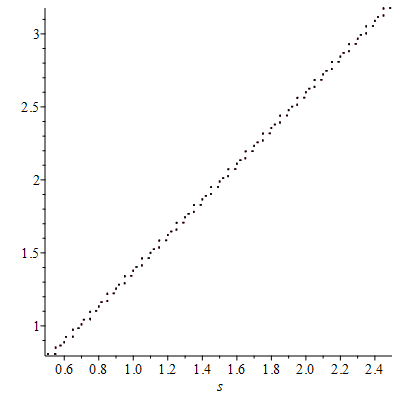
\includegraphics[width=1\linewidth]{../img/img1.png}}
	\end{minipage}
\end{figure}


Можем заметить, что графики совпали.


Оценим погрешность приближенного решения по методу Рунге-Кутты порядка $m=4$, используя практическое правило Рунге. Способ практической оценки абсолютной погрешности метода Рунге-Кутта порядка $m$ состоит в следующем:
\begin{enumerate}
	\item находят при фиксированном (доастаточно большом) $k \in \mathbb{N}$ приближенное табличное решение $^>\textbf{\underline{u}}_{(k)} = [u_0, u_1, \ldots, u_k>$ на сетке \\$A_k = \langle a=\tau_0, \tau_1, \ldots, \tau_k = b\rangle$ отрезка $[a;b]$; \\
	\item находят приближенное табличное решение $^>\textbf{\underline{u}}_{(k)}^* = [u_0^*, u_1^*, \ldots, u_k^*\rangle$ на сетке $\left\langle a=\tau_{0}, \frac{\tau_{0}+\tau_{1}}{2}, \tau_{1}, \frac{\tau_{1}+\tau_{2}}{2}, \tau_{2}, \ldots, \frac{\tau_{k-1}+\tau_{k}}{2}, \tau_{k}=b\right\rangle$ и, затем, составляют вектор\\ $^>\underset{\sim}{\textbf{u}}_{(k)}^* = [u_0^*, u_1^*, \ldots, u_k^*\rangle$;
	\item величину $\varepsilon = \frac{1}{2^m-1} || ^>\underset{\sim}{\textbf{u}}_{(k)} -  ^>\textbf{\underline{u}}_{(k)} ||$ считают практичекой погрешностью метода.
\end{enumerate}


Имеем:

\begin{equation*}
	|| ^>\underset{\sim}{\textbf{u}}_{(41)} -  ^>\textbf{\underline{u}}_{(41)} || = 0.06197620007
\end{equation*}




\textbf{Вывод.}\\
Таким образом, можем сделать вывод, что методы Рунге-Кутты порядка $m=4$, четырёхшаговый метод Адамса-Башфорта и метод прогноза-коррекции (с четвёртым порядком точности) могут успешно применяться для численного решения задачи Коши для нормальных ОДУ.





\end{document}